\JWlone{Evaluation}
\label{sec:evaluation}

What does it mean?


% #  ERROR OF ESTIMATION  ######################################################
\JWltwo{Error of Estimation}
\label{sec:error}

Presentation of measured and estimated work. Plus errors.


% #  COMPARISON TO SIMPLE TIME BASED MODEL  ####################################
\JWltwo{Comparison to a simple time based Model}
\label{sec:time-based}

This chapter features a comparison of the gained energy model to a simple
time-(only-)based one. See figures \ref{fig:errs-1cpu} and \ref{fig:errs-ncpu}.

\begin{figure}
  \centering
    \includegraphics[width=\textwidth]{fig/1cpu-bench-errs.eps}
  \caption{1 CPU error comparison}
  \label{fig:errs-1cpu}
\end{figure}

\begin{figure}
  \centering
    \includegraphics[width=\textwidth]{fig/Ncpu-bench-errs.eps}
  \caption{n CPU error comparison}
  \label{fig:errs-ncpu}
\end{figure}



% #  OVERHEAD IMPLEMENTATION  ##################################################
\JWltwo{Overhead of this Implementation}
\label{sec:overhead}

How many CPU clock cycles do I waste for the accounting the performance
counters.


% #  VARIATION BETWEEN RUNS  ###################################################
\JWltwo{Variation of Results between Runs}
\label{sec:variation}

Are there variations of the results between the runs?
